%% Chapter 17: Complexity Theory for Approximation and Parameterization
%% Status: drafted; all figures drawn.
%%
%% Written against "material/slides/FPT and Approximation Complexity.pptx"
%% (Johan van Rooij and Jesper Nederlof), 50 slides: parameterized complexity
%% and reductions on slides 1-30, approximation complexity on 31-50.
%%
%% The deck's parameterized half is a chain of four reductions ending at
%% dominating set; all four are given here in full.  The pool exercise --
%% Max Cut on multigraphs -- is not in the deck and is worked at the end.

\chapter[Complexity for Approximation and FPT]{Complexity Theory for Approximation and Parameterization}
\label{ch:hardness}

Every chapter of Parts~IV and~V has produced algorithms, and several have
gestured at limits: \cref{ch:approx-ii} said that maximum independent set has no
PTAS, \cref{ch:fpt-i} said that clique is $\mathrm{W}[1]$-complete and left the
class undefined. This chapter supplies the machinery behind both remarks. It is
about \emph{conditional non-existence proofs} --- how to show that an algorithm
of a given kind cannot exist unless something implausible is true --- in the two
settings where the classical theory has nothing to say: parameterized running
times, and approximation ratios.

The two halves share a shape. In each, one fixes a notion of reduction that
preserves the resource in question, identifies a problem that is complete for
the class under it, and then works outwards by reductions from there. That is
exactly what \textrm{NP}-completeness does for polynomial time, and the analogy
is worth keeping in view throughout.

\begin{goals}
  \poolgoal{explain what a conditional non-existence proof is, and say what an
        \textrm{NP}-hardness proof does and does not establish}
  \poolgoal{define $\mathrm{FPT}$, $\mathrm{XP}$ and the W-hierarchy, and
        explain why ``clique is not in $\mathrm{FPT}$'' is equivalent to
        $\mathrm{FPT} \ne \mathrm{W}[1]$}
  \poolgoal{define a parameterized reduction and prove that it transfers
        membership in $\mathrm{FPT}$}
  \poolgoal{explain why the standard polynomial reduction between independent
        set and vertex cover is not a parameterized reduction}
  \poolgoal{give the parameterized reduction from \lang{Clique} to
        \lang{Clique on Regular Graphs} and prove it correct}
  \poolgoal{give the parameterized reduction from \lang{Clique on Regular
        Graphs} to \lang{Multicoloured Clique} and prove it correct}
  \poolgoal{give the parameterized reduction from \lang{Multicoloured
        Independent Set} to \lang{Dominating Set} and explain what each gadget
        enforces}
  \poolgoal{define the class APX and APX-completeness, and state what the PCP
        theorem contributes}
  \poolgoal{define an L-reduction, and prove that L-reductions compose and
        preserve the existence of a PTAS}
  \poolgoal{give the L-reduction from \lang{Max 3-SAT} to \lang{Max 2-SAT} and
        conclude that \lang{Max 2-SAT} is APX-complete}
  \poolgoal{give the L-reduction from \lang{Max 2-SAT} to \lang{Maximum
        Independent Set} and conclude that it has no PTAS}
  \poolgoal{prove that \lang{Max Cut on Multigraphs} is APX-hard by an
        L-reduction from \lang{Max Not-All-Equal 3-SAT}}
\end{goals}

%==============================================================================
\section{Conditional non-existence proofs}
\label{sec:conditional-nonexistence}
%==============================================================================

It is worth being precise about what a hardness proof delivers, because
students routinely overstate it and researchers routinely understate it.

Proving a problem \textrm{NP}-complete does \emph{not} prove that it has no
polynomial-time algorithm. Nobody has proved that about any problem. What it
proves is a conditional statement:
\begin{quote}
  if $\mathrm{P} \ne \mathrm{NP}$, then this problem has no polynomial-time
  algorithm.
\end{quote}
Equivalently, and this is the more useful reading: \emph{a polynomial-time
algorithm for this problem would collapse $\mathrm{P}$ and $\mathrm{NP}$}. The
proof does not close the door; it attaches to the door a very large and very
public consequence.

That is the pattern of everything in this chapter and in
\cref{ch:lower-bounds}. Its value depends on two things --- how believable the
hypothesis is, and how many independent problems rest on it --- and on both
counts $\mathrm{P} \ne \mathrm{NP}$ does extremely well.

\begin{intuition}
The honest summary to give a student is: these proofs do not show that an
algorithm does not exist. They show that finding one would be a career-making
result requiring deep new insight, which is a different statement and is
usually the one that matters when deciding what to do on a Tuesday afternoon.
\end{intuition}

%==============================================================================
\section{The parameterized classes}
\label{sec:parameterized-classes}
%==============================================================================

\Cref{ch:fpt-i} defined $\mathrm{FPT}$ --- solvable in $f(k)\poly(n)$ time ---
and $\mathrm{XP}$ --- solvable in $\bigoh{n^{f(k)}}$ --- and observed that
these are genuinely different shapes of running time. Between them sits a
hierarchy.

\begin{definition}[The W-hierarchy]\label{def:w-hierarchy-again}
There are classes $\mathrm{W}[1], \mathrm{W}[2], \ldots$ with
\[ \mathrm{FPT} \subseteq \mathrm{W}[1] \subseteq \mathrm{W}[2] \subseteq
   \cdots \subseteq \mathrm{XP}, \]
defined by the depth of the Boolean circuits whose weighted satisfiability a
problem reduces to. We shall not use the definition, only the inclusions and
the fact that certain problems are complete for certain levels.
\end{definition}

The reason the definition can be skipped is the following, which is the
parameterized analogue of ``\lang{SAT} is \textrm{NP}-complete''.

\begin{theorem}[\citet{DowneyFellows2013}]\label{thm:clique-w1}
\lang{Clique}, parameterized by the size of the clique sought, is
$\mathrm{W}[1]$-complete. Consequently
\[ \lang{Clique} \in \mathrm{FPT}
   \quad\Longleftrightarrow\quad
   \mathrm{FPT} = \mathrm{W}[1]. \]
\end{theorem}

So the working hypothesis of parameterized complexity, $\mathrm{FPT} \ne
\mathrm{W}[1]$, can be stated without ever mentioning circuits: \emph{there is
no algorithm finding a $k$-clique in $f(k)\poly(n)$ time}. Everything in the
first half of this chapter is a conditional non-existence proof under that
hypothesis.

\begin{remark}\label{rem:w1-vs-pnp}
How does $\mathrm{FPT} \ne \mathrm{W}[1]$ compare with
$\mathrm{P} \ne \mathrm{NP}$? It is the stronger assumption: if
$\mathrm{P} = \mathrm{NP}$ then clique is solvable in polynomial time and hence
certainly in $f(k)\poly(n)$ time, so $\mathrm{FPT} = \mathrm{W}[1]$. Assuming
$\mathrm{FPT} \ne \mathrm{W}[1]$ therefore assumes
$\mathrm{P} \ne \mathrm{NP}$ and more.
\end{remark}

%==============================================================================
\section{Parameterized reductions}
\label{sec:parameterized-reductions}
%==============================================================================

A polynomial-time reduction is the wrong tool here, and seeing exactly why is
the point of this section.

\begin{definition}[Parameterized reduction]\label{def:parameterized-reduction}
A \emph{parameterized reduction} from a parameterized problem $A$ to a
parameterized problem $B$ is an algorithm $R$ mapping an instance $(x,k)$ of
$A$ to an instance $(x',k')$ of $B$ such that
\begin{enumerate}[label=(\roman*),leftmargin=*,nosep]
  \item $(x,k)$ is a yes-instance if and only if $(x',k')$ is;
  \item $k' \le g(k)$ for some computable function $g$;
  \item $R$ runs in $f(k)\poly(|x|)$ time for some computable function $f$.
\end{enumerate}
\end{definition}

Condition (ii) is the one that is new, and it is the whole difficulty: the new
parameter must be bounded by a function of the old one \emph{alone}, with no
dependence on the instance size.

\begin{lemma}\label{lem:param-reduction-works}
If there is a parameterized reduction from $A$ to $B$ and $B \in \mathrm{FPT}$,
then $A \in \mathrm{FPT}$. Contrapositively, if $A \notin \mathrm{FPT}$ then
$B \notin \mathrm{FPT}$.
\end{lemma}

\begin{proof}
Let $R$ run in $f(k)\poly(|x|)$ time and let $B$ be solvable in
$h(k')\poly(|x'|)$ time. Given $(x,k)$, run $R$; this costs
$f(k)\poly(|x|)$, and since an algorithm cannot write more output than it takes
steps, $|x'| \le f(k)\poly(|x|)$. Now run the algorithm for $B$ on $(x',k')$,
at cost
\[ h(k')\poly(|x'|) \;\le\; h(g(k)) \cdot \poly\bigl(f(k)\poly(|x|)\bigr)
   \;\le\; h(g(k)) f(k)^{c} \cdot \poly(|x|), \]
because a polynomial of $f(k)\poly(|x|)$ is a function of $k$ times a
polynomial of $|x|$. The total is of the form $f'(k)\poly(|x|)$.
\end{proof}

\subsection{Independent set}

\begin{proposition}\label{prop:is-not-fpt}
Assuming $\mathrm{FPT} \ne \mathrm{W}[1]$, \lang{Independent Set} parameterized
by the size of the set is not in $\mathrm{FPT}$.
\end{proposition}

\begin{proof}
Reduce from \lang{Clique}: given $(G,k)$, output $(\bar G, k)$, where $\bar G$
is the complement. A set of vertices is a clique in $G$ if and only if it is
independent in $\bar G$, so (i) holds; $k' = k$, so (ii) holds with
$g(k) = k$; and complementing a graph is polynomial, so (iii) holds. Apply
\cref{lem:param-reduction-works} and \cref{thm:clique-w1}.
\end{proof}

\subsection{Why vertex cover does not follow}

Now the instructive failure. A set $I$ is independent in $G = (V,E)$ if and only
if $V \setminus I$ is a vertex cover, so \lang{Independent Set} reduces to
\lang{Vertex Cover} in polynomial time: ask for a vertex cover of size $n-k$.
And yet \cref{ch:fpt-i} solved \lang{Vertex Cover} in $\bigoh{2^k(n+m)}$ time,
so it \emph{is} in $\mathrm{FPT}$, and by
\cref{lem:param-reduction-works} that would put independent set in
$\mathrm{FPT}$ too, contradicting \cref{prop:is-not-fpt}.

The resolution is condition (ii). The new parameter is $n-k$, which is not
bounded by any function of $k$ --- it grows with the instance. So the reduction
is a perfectly good polynomial-time reduction and not a parameterized one.

\begin{intuition}
This is the single most important thing to take from the first half of the
chapter. In classical complexity all \textrm{NP}-complete problems are
interreducible, so hardness proofs may travel in any direction. In
parameterized complexity the parameter has to be carried along, and a reduction
that mangles it is worthless. Independent set and vertex cover are the same
problem up to complementation and sit on opposite sides of the
$\mathrm{FPT}$ boundary; the parameter is the entire difference.
\end{intuition}

%==============================================================================
\section{A chain of reductions}
\label{sec:reduction-chain}
%==============================================================================

We now build a chain from \lang{Clique} to \lang{Dominating Set}, in three
steps. Each step is a small construction; the value of the chain is that the
intermediate problems, especially the multicoloured ones, are far more
convenient starting points for later reductions than clique itself.

\subsection{Making the graph regular}

\begin{probdef}{Clique on Regular Graphs}
  \instance A graph $G = (V,E)$ in which every vertex has the same degree $d$.
  \parameter An integer $k$.
  \question Does $G$ have a clique of size at least $k$?
\end{probdef}

\begin{lemma}\label{lem:clique-regular}
There is a parameterized reduction from \lang{Clique} to \lang{Clique on
Regular Graphs}.
\end{lemma}

\begin{proof}
Let $(G,k)$ be given. If $k \le 2$ the question is trivial --- a $1$-clique is a
vertex and a $2$-clique an edge --- so answer it directly and output a fixed
trivial instance. Assume $k \ge 3$.

Let $d$ be the maximum degree of $G$. Construct $G'$ as follows.
\begin{itemize}[leftmargin=*,nosep]
  \item Take $d$ disjoint copies $G_1, \ldots, G_d$ of $G$, writing $v_i$ for
        the copy of $v$ in $G_i$.
  \item For every $v \in V$, add $d - \deg(v)$ new vertices, each joined to all
        $d$ copies $v_1, \ldots, v_d$ of $v$ and to nothing else.
\end{itemize}
Set $k' = k$.

\emph{$G'$ is $d$-regular.} A copy $v_i$ has $\deg(v)$ neighbours inside $G_i$
and is joined to each of the $d - \deg(v)$ new vertices belonging to $v$, for a
total of $d$. A new vertex is joined to exactly the $d$ copies of its vertex.

\emph{Correctness.} If $G$ has a $k$-clique then so does $G_1 \subseteq G'$.
Conversely, suppose $G'$ has a clique $K$ with $|K| = k \ge 3$. No new vertex
lies in a triangle: the neighbourhood of a new vertex is $\{v_1,\ldots,v_d\}$,
and these lie in pairwise disjoint copies, so no two of them are adjacent.
Hence $K$ contains no new vertex. The copies are pairwise disconnected once the
new vertices are removed, so $K$ lies inside a single $G_i$ and is a $k$-clique
of $G$.

\emph{It is a parameterized reduction.} $k' = k$, so (ii) holds, and the
construction is polynomial in $|G|$, so (iii) holds.
\end{proof}

\begin{figure}[ht]
\centering
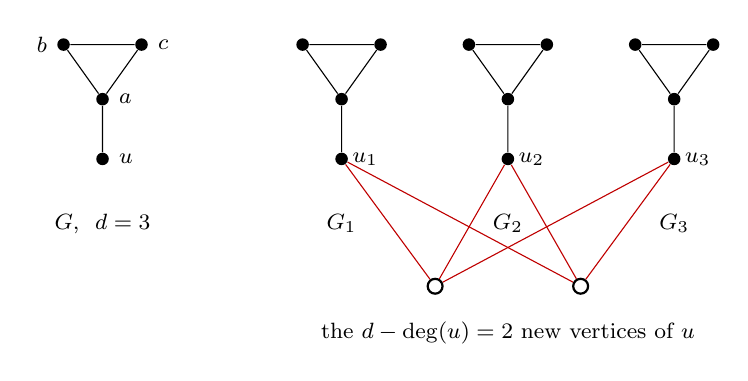
\begin{tikzpicture}[scale=0.66,
    vtx/.style={circle,fill=black,inner sep=1.6pt},
    new/.style={circle,draw,thick,fill=white,inner sep=1.9pt},
    ne/.style={red!75!black},
    every node/.style={font=\footnotesize}]
  % ---- the input graph, of maximum degree three ----
  \begin{scope}[xshift=-3.4cm]
    \node[vtx,label=right:$a$] (a) at (0,0) {};
    \node[vtx,label=left:$b$]  (b) at (-0.75,1.05) {};
    \node[vtx,label=right:$c$] (c) at (0.75,1.05) {};
    \node[vtx,label=right:$u$] (u) at (0,-1.15) {};
    \draw (a)--(b)--(c)--(a) (a)--(u);
    \node at (0,-2.4) {$G$, \ $d = 3$};
  \end{scope}
  % ---- three disjoint copies ----
  \foreach \i/\dx in {1/1.2, 2/4.4, 3/7.6}{
    \begin{scope}[xshift=\dx cm]
      \node[vtx] (a\i) at (0,0) {};
      \node[vtx] (b\i) at (-0.75,1.05) {};
      \node[vtx] (c\i) at (0.75,1.05) {};
      \node[vtx,label={[label distance=-2pt]right:$u_\i$}] (u\i) at (0,-1.15) {};
      \draw (a\i)--(b\i)--(c\i)--(a\i) (a\i)--(u\i);
      \node[fill=white,inner sep=1.5pt] at (0,-2.4) {$G_\i$};
    \end{scope}
  }
  % ---- the new vertices belonging to u ----
  \node[new] (n1) at (3.0,-3.6) {};
  \node[new] (n2) at (5.8,-3.6) {};
  \foreach \i in {1,2,3}{ \draw[ne] (n1)--(u\i); \draw[ne] (n2)--(u\i); }
  \node at (4.4,-4.5) {the $d - \deg(u) = 2$ new vertices of $u$};
\end{tikzpicture}
\caption{The construction of \cref{lem:clique-regular}. The new vertices top up
every degree to $d$, and they are useless to a clique because their
neighbourhoods are independent. Only the two new vertices belonging to $u$ are
drawn; $b$ and $c$ have one each, and $a$, already of degree $3$, has none.}
\label{fig:clique-regular}
\end{figure}

\subsection{Adding colours}

\begin{probdef}{Multicoloured Clique}
  \instance A graph $G = (V,E)$ together with a partition of $V$ into $k$
  colour classes $V_1, \ldots, V_k$.
  \parameter An integer $k$.
  \question Does $G$ have a clique of size $k$ containing exactly one vertex of
  each colour?
\end{probdef}

\begin{lemma}\label{lem:multicoloured-clique}
There is a parameterized reduction from \lang{Clique on Regular Graphs} to
\lang{Multicoloured Clique on Regular Graphs}.
\end{lemma}

\begin{proof}
Let $G$ be $d$-regular with parameter $k$. Construct $G'$:
\begin{itemize}[leftmargin=*,nosep]
  \item for every $v \in V$ create $k$ vertices $v^1, \ldots, v^k$, giving
        $v^i$ the colour $i$;
  \item join $v^i$ and $u^j$ exactly when $i \ne j$ and $uv \in E$.
\end{itemize}
Set $k' = k$.

\emph{$G'$ is regular.} The vertex $v^i$ is joined to $u^j$ for each of the $d$
neighbours $u$ of $v$ and each of the $k-1$ colours $j \ne i$, so every vertex
has degree $(k-1)d$.

\emph{Correctness.} If $\{v_1,\ldots,v_k\}$ is a clique of $G$, then
$\{v_1^1, v_2^2, \ldots, v_k^k\}$ is a multicoloured clique of $G'$: any two of
its vertices have different colours and their underlying vertices are adjacent.

Conversely let $\{v_1^1, \ldots, v_k^k\}$ be a multicoloured $k$-clique. For
$i \ne j$ the vertices $v_i^i$ and $v_j^j$ are adjacent, so $v_iv_j \in E$; in
particular $v_i \ne v_j$, since $G$ has no loops. So $\{v_1,\ldots,v_k\}$ is a
$k$-clique of $G$.

Again $k' = k$ and the construction is polynomial.
\end{proof}

Dropping the regularity gives \lang{Multicoloured Clique}, and complementing
\emph{within and between} colour classes appropriately gives
\lang{Multicoloured Independent Set}; both are therefore not in $\mathrm{FPT}$
under the hypothesis. \Cref{ex:multicoloured-is} asks you to write the second
of these down.

\begin{intuition}
Why bother with colours? Because a reduction \emph{from} multicoloured clique
starts with far more structure to work with: the solution is known in advance to
take exactly one vertex from each of $k$ named groups. Gadgets can then be built
per group and per pair of groups, which is what the next reduction does and what
almost every $\mathrm{W}[1]$-hardness proof in the literature does. Adding
structure to the source problem is work done once and reused for ever.
\end{intuition}

\subsection{Dominating set}

\begin{probdef}{Dominating Set}
  \instance A graph $G = (V,E)$.
  \parameter An integer $k$.
  \question Is there a set $D$ of at most $k$ vertices such that every vertex
  is in $D$ or adjacent to a vertex of $D$?
\end{probdef}

\begin{theorem}\label{thm:dominating-set-w2}
There is a parameterized reduction from \lang{Multicoloured Independent Set} to
\lang{Dominating Set}. Hence, assuming $\mathrm{FPT} \ne \mathrm{W}[1]$,
\lang{Dominating Set} is not in $\mathrm{FPT}$.
\end{theorem}

\begin{proof}
Let $G = (V,E)$ with colour classes $V_1, \ldots, V_k$ and parameter $k$ be
given. Build $H$:
\begin{itemize}[leftmargin=*]
  \item one vertex per vertex of $G$, with every colour class $V_i$ turned into
        a \emph{clique};
  \item for each $i$, two new vertices $x_i$ and $y_i$, each joined to every
        vertex of $V_i$ and not to each other;
  \item for each edge $\{u,v\} \in E$ with $u \in V_i$, $v \in V_j$ and
        $i \ne j$, a new vertex $w_{uv}$ joined to every vertex of
        $V_i \cup V_j$ \emph{except} $u$ and $v$.
\end{itemize}
Set $k' = k$.

\emph{One vertex per class.} Consider any dominating set $D$ of $H$ with
$|D| \le k$. The closed neighbourhoods of $x_i$ and of $y_i$ are
$\{x_i\} \cup V_i$ and $\{y_i\} \cup V_i$, which meet only in $V_i$. So
dominating both $x_i$ and $y_i$ costs either one vertex of $V_i$ or two
vertices. Since there are $k$ classes and only $k$ vertices to spend, $D$ must
contain exactly one vertex of each $V_i$ and nothing else.

\emph{Independence.} Write $D = \{s_1, \ldots, s_k\}$ with $s_i \in V_i$, and
suppose $\{s_i, s_j\} \in E$ for some $i \ne j$. The vertex $w_{s_is_j}$ is
joined to every vertex of $V_i \cup V_j$ except $s_i$ and $s_j$, and to nothing
outside $V_i \cup V_j$; and $D \cap (V_i \cup V_j) = \{s_i,s_j\}$. So
$w_{s_is_j}$ is neither in $D$ nor adjacent to it, contradicting domination.
Hence $D$ is a multicoloured independent set of size $k$.

\emph{Conversely}, let $S = \{s_1,\ldots,s_k\}$ be a multicoloured independent
set of $G$. Each $s_i$ dominates all of $V_i$, because $V_i$ is a clique in $H$,
and also $x_i$ and $y_i$. For a vertex $w_{uv}$ with $u \in V_i$, $v \in V_j$:
if $s_i \ne u$ then $w_{uv}$ is adjacent to $s_i$; and if $s_i = u$ then, since
$S$ is independent and $\{u,v\} \in E$, we have $s_j \ne v$, so $w_{uv}$ is
adjacent to $s_j$. Either way $w_{uv}$ is dominated. So $S$ is a dominating set
of $H$ of size $k$.
\end{proof}

\begin{figure}[ht]
\centering
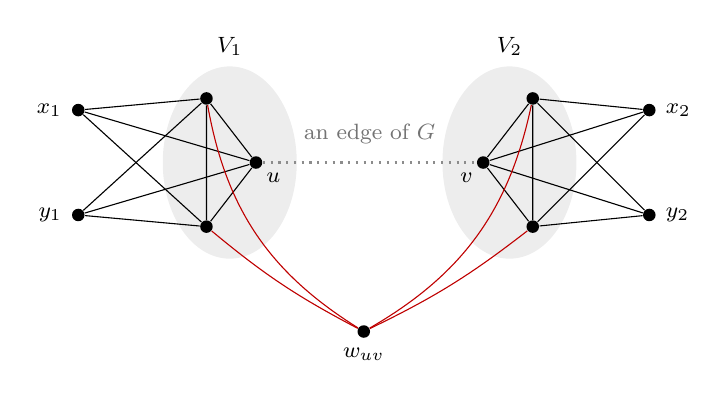
\begin{tikzpicture}[scale=0.74,
    vtx/.style={circle,fill=black,inner sep=1.6pt},
    wed/.style={red!75!black},
    every node/.style={font=\footnotesize}]
  % the two colour classes, each a clique in H
  \fill[black!7] (0.3,0) ellipse (1.15 and 1.65);
  \fill[black!7] (5.1,0) ellipse (1.15 and 1.65);
  \node at (0.3,2.0) {$V_1$};
  \node at (5.1,2.0) {$V_2$};
  \node[vtx] (a1) at (-0.1,1.1) {};
  \node[vtx,label={[label distance=-2pt]below right:$u$}] (u) at (0.75,0) {};
  \node[vtx] (a3) at (-0.1,-1.1) {};
  \node[vtx] (b2) at (5.5,1.1) {};
  \node[vtx,label={[label distance=-2pt]below left:$v$}] (v) at (4.65,0) {};
  \node[vtx] (b3) at (5.5,-1.1) {};
  \draw (a1)--(u)--(a3)--(a1);
  \draw (b2)--(v)--(b3)--(b2);
  % the forcing pairs
  \node[vtx,label=left:$x_1$] (x1) at (-2.3,0.9) {};
  \node[vtx,label=left:$y_1$] (y1) at (-2.3,-0.9) {};
  \node[vtx,label=right:$x_2$] (x2) at (7.5,0.9) {};
  \node[vtx,label=right:$y_2$] (y2) at (7.5,-0.9) {};
  \foreach \z in {x1,y1}{ \draw (\z)--(a1) (\z)--(u) (\z)--(a3); }
  \foreach \z in {x2,y2}{ \draw (\z)--(b2) (\z)--(v) (\z)--(b3); }
  % the edge of G that the w vertex is built from -- it is not an edge of H
  \draw[black!45,dotted,thick] (u)--(v)
        node[midway,above=3pt,black!55] {an edge of $G$};
  % the w vertex: joined to everything in V_1 cup V_2 except u and v
  \node[vtx,label=below:$w_{uv}$] (w) at (2.6,-2.9) {};
  \draw[wed] (w) to[bend left=24] (a1);
  \draw[wed] (w) to[bend left=6] (a3);
  \draw[wed] (w) to[bend right=24] (b2);
  \draw[wed] (w) to[bend right=6] (b3);
\end{tikzpicture}
\caption{The gadgets of \cref{thm:dominating-set-w2}. The pair $x_i,y_i$ forces
exactly one vertex to be chosen from each class; the vertex $w_{uv}$ is left
undominated exactly when both ends of the edge $uv$ are chosen.}
\label{fig:dominating-set-gadget}
\end{figure}

\begin{remark}[Where the chain stops]\label{rem:w1-w2}
Stacking the three reductions gives a parameterized reduction from independent
set to dominating set. There is no reduction back, and this is not for want of
trying: independent set is $\mathrm{W}[1]$-complete and dominating set is
$\mathrm{W}[2]$-complete, and $\mathrm{W}[1] \subseteq \mathrm{W}[2]$ is
believed to be strict.

That is a real difference from classical complexity, where every
\textrm{NP}-complete problem reduces to every other and the notion of ``harder''
does not arise. Parameterized complexity has levels, and it is worth knowing
which level a problem sits on even if the definition of the levels is left in
the textbook.
\end{remark}

%==============================================================================
\section{APX and APX-completeness}
\label{sec:apx-completeness}
%==============================================================================

Now the second half, and the same shape again.

\Cref{ch:approx-ii} laid out five qualities of approximation and gave two
techniques for showing that a problem does not have one --- the gap technique
and the polynomial-bound technique. Neither of them can do the following job:
show that a problem with a constant-factor approximation has \emph{no} PTAS.
The gap technique separates constant ratios from none at all; the
polynomial-bound technique separates FPTAS from PTAS. Between APX and PTAS
there is a gap in the toolkit, and a completeness theory fills it.

\begin{definition}[APX-completeness]\label{def:apx-complete}
A problem is \emph{APX-hard} if every problem in APX reduces to it by a
reduction preserving the existence of a PTAS, and \emph{APX-complete} if it is
also in APX. Consequently, if one APX-complete problem has a PTAS then all of
them do.
\end{definition}

\begin{theorem}[PCP theorem, \citet{AroraSafra1998,AroraLundMotwaniSudanSzegedy1998}]
\label{thm:pcp}
\lang{Max 3-SAT} is APX-complete. Consequently no APX-complete problem has a
PTAS unless $\mathrm{P} = \mathrm{NP}$.
\end{theorem}

We do not prove this --- it is one of the deepest theorems in complexity theory
--- but the role it plays is exactly Cook's: it supplies the first complete
problem, and everything afterwards is a reduction.

\begin{center}
\begin{tabular}{@{}p{0.46\textwidth}p{0.46\textwidth}@{}}
\toprule
\textbf{Classical} & \textbf{Approximation} \\
\midrule
if one \textrm{NP}-complete problem is in $\mathrm{P}$, all are
  & if one APX-complete problem has a PTAS, all do \\
\addlinespace
polynomial-time reductions & L-reductions \\
\addlinespace
Cook: \lang{SAT} is \textrm{NP}-complete
  & PCP: \lang{Max 3-SAT} is APX-complete \\
\bottomrule
\end{tabular}
\end{center}

%==============================================================================
\section{L-reductions}
\label{sec:l-reductions}
%==============================================================================

The reduction that preserves approximability is the following. Write
$\OPT(x)$ for the optimum value of an instance $x$ and $\mathrm{VAL}(y)$ for the
value of a solution $y$.

\begin{definition}[L-reduction]\label{def:l-reduction}
$P_1$ \emph{L-reduces} to $P_2$, written $P_1 \le_L P_2$, if there are
polynomial-time computable functions $f$ and $g$ --- $f$ mapping instances of
$P_1$ to instances of $P_2$, and $g$ mapping solutions of $f(x)$ back to
solutions of $x$ --- and constants $a, b > 0$ such that for every instance $x$
of $P_1$ and every solution $y$ of $f(x)$:
\begin{align}
  \OPT(f(x)) &\;\le\; a \cdot \OPT(x), \label{eq:lred-a}\\
  \bigl|\OPT(x) - \mathrm{VAL}(g(y))\bigr|
    &\;\le\; b \cdot \bigl|\OPT(f(x)) - \mathrm{VAL}(y)\bigr|.
    \label{eq:lred-b}
\end{align}
\end{definition}

Read \eqref{eq:lred-a} as: the reduction does not inflate the optimum, so a
relative error in $P_2$ is still a relative error in $P_1$. Read
\eqref{eq:lred-b} as: the reduction does not amplify absolute error --- a
solution that is $\varepsilon$ away from optimal in the image comes back at
most $b\varepsilon$ away from optimal in the source.

\begin{theorem}\label{thm:lred-preserves-ptas}
If $P_1 \le_L P_2$ and $P_2$ has a PTAS, then $P_1$ has a PTAS.
\end{theorem}

\begin{proof}
Let $\varepsilon' > 0$ be the ratio wanted for $P_1$, and put
$\varepsilon = \varepsilon'/(ab)$. Given an instance $x$ of $P_1$, compute
$f(x)$, run the PTAS for $P_2$ on it with parameter $\varepsilon$ to get a
solution $y$, and return $g(y)$. Then
\begin{align*}
  \bigl|\OPT(x) - \mathrm{VAL}(g(y))\bigr|
    &\;\le\; b\,\bigl|\OPT(f(x)) - \mathrm{VAL}(y)\bigr|
      && \text{by \eqref{eq:lred-b}} \\
    &\;\le\; b\,\varepsilon\, \OPT(f(x))
      && \text{since $y$ is within $1+\varepsilon$} \\
    &\;\le\; a\,b\,\varepsilon\, \OPT(x)
      && \text{by \eqref{eq:lred-a}} \\
    &\;=\; \varepsilon' \OPT(x).
\end{align*}
So $\mathrm{VAL}(g(y))$ is within a factor $1+\varepsilon'$ of $\OPT(x)$. Every
step is polynomial for fixed $\varepsilon'$.
\end{proof}

\begin{lemma}\label{lem:lred-composes}
If $P_1 \le_L P_2$ with constants $a_1, b_1$ and $P_2 \le_L P_3$ with constants
$a_2, b_2$, then $P_1 \le_L P_3$ with constants $a_1a_2$ and $b_1b_2$.
\end{lemma}

\begin{proof}
Compose the maps: $f = f_2 \circ f_1$ and $g = g_1 \circ g_2$. Then
$\OPT(f_2(f_1(x))) \le a_2 \OPT(f_1(x)) \le a_2a_1\OPT(x)$, and applying
\eqref{eq:lred-b} twice gives the second constant.
\end{proof}

So APX-hardness proofs may be chained, exactly as \textrm{NP}-hardness proofs
are. To prove a problem APX-complete: give a constant-factor approximation, and
give an L-reduction from a problem already known to be APX-hard.

%==============================================================================
\section{Max 2-SAT is APX-complete}
\label{sec:max2sat-apx}
%==============================================================================

The first link in the chain, starting from \cref{thm:pcp}.

\begin{theorem}\label{thm:max3sat-max2sat}
$\lang{Max 3-SAT} \le_L \lang{Max 2-SAT}$, with $a = 13$ and $b = 1$.
\end{theorem}

\begin{proof}
\emph{The map $f$.} Replace each clause $(x \vee y \vee z)$ of the input by the
following ten clauses of at most two literals, where $v$ is a fresh variable
used by this clause only:
\[ (x),\ (y),\ (z),\ (v),\
   (\neg x \vee \neg y),\ (\neg x \vee \neg z),\ (\neg y \vee \neg z),\
   (x \vee \neg v),\ (y \vee \neg v),\ (z \vee \neg v). \]
\emph{The map $g$.} Restrict a truth assignment of $f(I)$ to the original
variables, forgetting the $v$'s.

\emph{The key computation.} Check the truth table of the ten clauses against
the eight assignments of $x,y,z$, choosing $v$ to maximise. If at least one of
$x,y,z$ is true, the best choice of $v$ satisfies exactly $7$ of the ten; if all
three are false, it satisfies exactly $6$. So for any assignment $\varphi$ of
the original variables, extended optimally,
\[ \mathrm{VAL}(f\text{-assignment}) \;=\; 6|C| + \#\{\text{clauses of } I
   \text{ satisfied by } \varphi\}, \]
and in particular $\OPT(f(I)) = 6|C| + \OPT(I)$.

\emph{Condition \eqref{eq:lred-a}.} Some assignment satisfies at least half the
clauses of $I$ --- take the better of an assignment and its negation, as in
\cref{thm:maxsat} --- so $\OPT(I) \ge |C|/2$, that is $6|C| \le 12\OPT(I)$.
Hence
\[ \OPT(f(I)) \;=\; 6|C| + \OPT(I) \;\le\; 12\OPT(I) + \OPT(I)
   \;=\; 13\,\OPT(I). \]

\emph{Condition \eqref{eq:lred-b}.} For any assignment $y$ of $f(I)$ we have
$\mathrm{VAL}(y) \le 6|C| + \mathrm{VAL}(g(y))$, by the same truth table --- a
clause of $I$ satisfied by $g(y)$ contributes at most $7$ and an unsatisfied one
at most $6$. Therefore
\[ \OPT(f(I)) - \mathrm{VAL}(y)
   \;\ge\; \bigl(6|C| + \OPT(I)\bigr) - \bigl(6|C| + \mathrm{VAL}(g(y))\bigr)
   \;=\; \OPT(I) - \mathrm{VAL}(g(y)), \]
which is \eqref{eq:lred-b} with $b = 1$.
\end{proof}

\begin{corollary}\label{cor:max2sat-apx-complete}
\lang{Max 2-SAT} is APX-complete, and therefore has no PTAS unless
$\mathrm{P} = \mathrm{NP}$.
\end{corollary}

\begin{proof}
APX-hard by \cref{thm:max3sat-max2sat} and \cref{thm:pcp}; in APX because the
$2$-approximation for \lang{Max SAT} of \cref{thm:maxsat} applies to it.
\end{proof}

%==============================================================================
\section{Maximum independent set has no PTAS}
\label{sec:mis-no-ptas}
%==============================================================================

\Cref{ch:approx-ii} showed that maximum independent set admits no absolute
constant difference approximation and no FPTAS, and asserted --- forward to this
chapter --- that it has no PTAS either. Here is the proof.

\begin{theorem}\label{thm:max2sat-mis}
$\lang{Max 2-SAT} \le_L \lang{Maximum Independent Set}$, with $a = b = 1$.
Hence maximum independent set is APX-hard.
\end{theorem}

\begin{proof}
\emph{The map $f$.} For each clause of the input create one vertex per literal
of that clause, and join the vertices of the same clause to each other. Then, for
every variable $x$, join every vertex labelled $x$ to every vertex labelled
$\neg x$.

\emph{The map $g$.} Given an independent set $S$, set a variable $x$ to true if
$S$ contains a vertex labelled $x$, to false if it contains one labelled
$\neg x$, and arbitrarily if neither.

\emph{$g$ is well defined and $\OPT(f(I)) = \OPT(I)$.} An independent set
contains at most one vertex per clause, since each clause is a clique, and never
both an $x$-vertex and a $\neg x$-vertex, since those are joined. So $S$
describes a consistent partial assignment together with, for each vertex of $S$,
a clause that assignment satisfies; hence $g(S)$ satisfies at least $|S|$
clauses, giving $\mathrm{VAL}(g(S)) \ge \mathrm{VAL}(S)$. Conversely an
assignment satisfying $s$ clauses yields an independent set of size $s$ --- pick
one satisfied literal from each satisfied clause --- so the two optima are equal
and \eqref{eq:lred-a} holds with $a = 1$.

\emph{Condition \eqref{eq:lred-b}.} Using $\OPT(f(I)) = \OPT(I)$ and
$\mathrm{VAL}(g(S)) \ge \mathrm{VAL}(S)$,
\[ \OPT(I) - \mathrm{VAL}(g(S)) \;\le\; \OPT(f(I)) - \mathrm{VAL}(S), \]
so $b = 1$.
\end{proof}

\begin{corollary}\label{cor:mis-no-ptas}
Unless $\mathrm{P} = \mathrm{NP}$, maximum independent set has no PTAS. With
\cref{thm:is-not-apx} it follows that maximum independent set is not in APX at
all.
\end{corollary}

\begin{proof}
The first statement is \cref{thm:max2sat-mis}, \cref{cor:max2sat-apx-complete}
and \cref{thm:lred-preserves-ptas}. For the second, \cref{thm:is-not-apx} says
that a constant-factor approximation for maximum independent set would yield a
PTAS, which the first statement forbids.
\end{proof}

That closes the loop opened in \cref{ch:approx-ii}: the self-reduction there
turned ``in APX'' into ``has a PTAS'', and the L-reduction here rules out the
PTAS. Neither half suffices alone.

%==============================================================================
\section{Max cut on multigraphs}
\label{sec:max-cut-apx}
%==============================================================================

The chapter's pool exercise. It is a second L-reduction, from a different
starting point, and the gadgets are pleasantly concrete.

\begin{probdef}{Max Not-All-Equal 3-SAT}
  \instance A set of clauses over variables $X$, each clause containing exactly
  two or three literals.
  \question A truth assignment maximising the number of clauses that contain at
  least one true and at least one false literal.
\end{probdef}

\begin{probdef}{Max Cut on Multigraphs}
  \instance A multigraph $G = (V,E)$, in which an edge may appear several
  times.
  \question A partition of $V$ into $V_1, V_2$ maximising the number of edges
  with one endpoint in each.
\end{probdef}

We take as given that \lang{Max Not-All-Equal 3-SAT} is APX-complete.

\begin{theorem}\label{thm:maxcut-apx-hard}
$\lang{Max Not-All-Equal 3-SAT} \le_L \lang{Max Cut on Multigraphs}$, with
$a = 14$ and $b = 1/2$. Hence \lang{Max Cut on Multigraphs} is APX-hard.
\end{theorem}

\begin{proof}
Let $I$ have clause set $C$ and variables $X$, and write $\occ(x)$ for the
number of occurrences of the variable $x$, counting both polarities.

\emph{The map $f$.} The multigraph $G$ has one vertex per literal --- so two
vertices $x$ and $\neg x$ per variable --- and the following edges.
\begin{itemize}[leftmargin=*,nosep]
  \item \emph{Consistency.} For each variable $x$, put $2\occ(x)$ parallel
        edges between the vertices $x$ and $\neg x$.
  \item \emph{Clauses.} For a clause with three literals
        $\ell_1, \ell_2, \ell_3$, add the three edges
        $\ell_1\ell_2, \ell_2\ell_3, \ell_1\ell_3$. For a clause with two
        literals $\ell_1, \ell_2$, add \emph{two} parallel edges
        $\ell_1\ell_2$.
\end{itemize}

Call a cut \emph{consistent} if $x$ and $\neg x$ lie on opposite sides for
every variable. A consistent cut is exactly a truth assignment: put the true
literals in $V_1$. Writing $W = \sum_{x \in X} 2\occ(x)$ for the number of
consistency edges, a consistent cut cuts all of them, and

\begin{itemize}[leftmargin=*,nosep]
  \item a three-literal clause contributes $2$ if its literals are not all on
        the same side and $0$ otherwise --- a triangle is cut in two edges or
        in none;
  \item a two-literal clause contributes $2$ if its two literals are on
        opposite sides and $0$ otherwise.
\end{itemize}
Both gadgets therefore contribute $2$ exactly when the clause is
not-all-equal-satisfied, which is why the two-literal gadget was doubled. Hence
for the assignment $\varphi$ corresponding to a consistent cut,
\begin{equation}\label{eq:maxcut-value}
  \mathrm{VAL}(\text{cut}) \;=\; W + 2\,s(\varphi),
\end{equation}
where $s(\varphi)$ is the number of clauses $\varphi$ satisfies.

\emph{The map $g$: making a cut consistent.} Given any cut, repeat: if $x$ and
$\neg x$ lie on the same side, move the vertex $x$ to the other side. This gains
the $2\occ(x)$ consistency edges, which were uncut. It loses at most the clause
edges at $x$, and $x$ has at most $2\occ_{+}(x) \le 2\occ(x)$ of those --- each
clause containing the literal $x$ contributes two edges at $x$, whether it has
two literals or three. So the value never decreases. Each step fixes one
variable and disturbs no other, so at most $|X|$ steps are needed. Let $g$
output the assignment read off the resulting consistent cut.

\emph{Condition \eqref{eq:lred-a}.} By the above, some optimal cut is
consistent, so $\OPT(f(I)) = W + 2\OPT(I)$ by \eqref{eq:maxcut-value}. A random
assignment satisfies a two-literal clause with probability $1/2$ and a
three-literal clause with probability $3/4$, so $\OPT(I) \ge |C|/2$. Each clause
has at most three literals, so the total number of literal occurrences is at
most $3|C|$ and
\[ W \;=\; 2\sum_{x} \occ(x) \;\le\; 6|C| \;\le\; 12\,\OPT(I). \]
Hence $\OPT(f(I)) \le 12\OPT(I) + 2\OPT(I) = 14\,\OPT(I)$.

\emph{Condition \eqref{eq:lred-b}.} For any cut $y$, making it consistent does
not decrease its value, so $\mathrm{VAL}(y) \le W + 2\,\mathrm{VAL}(g(y))$.
Therefore
\[ \OPT(f(I)) - \mathrm{VAL}(y)
   \;\ge\; \bigl(W + 2\OPT(I)\bigr) - \bigl(W + 2\mathrm{VAL}(g(y))\bigr)
   \;=\; 2\bigl(\OPT(I) - \mathrm{VAL}(g(y))\bigr), \]
which is \eqref{eq:lred-b} with $b = 1/2$.
\end{proof}

\begin{intuition}
Two design decisions carried this proof, and both are worth stealing. The
two-literal gadget was \emph{doubled} so that every satisfied clause contributes
the same amount; without that the objective would be a weighted count and the
error bound \eqref{eq:lred-b} would not survive. And the consistency
multiplicity was set to $2\occ(x)$ --- large enough that inconsistency never
pays, small enough that $W$ stays proportional to $|C|$ and hence to $\OPT(I)$.
A larger multiplicity would still force consistency but would destroy
\eqref{eq:lred-a}, because $a$ has to be a constant.
\end{intuition}

%==============================================================================
\section{Notes and further reading}
\label{sec:hardness-further-reading}
%==============================================================================

This chapter follows the lecture slides of Johan van Rooij and Jesper Nederlof.

For the parameterized half, \citet{DowneyFellows2013} is the source of the
W-hierarchy and of \cref{thm:clique-w1}, and
\citet[Chapter~13]{CyganEtAl2015} is the modern textbook account of
$\mathrm{W}[1]$-hardness proofs, including the multicoloured technique used in
\cref{sec:reduction-chain}.

For the approximation half, L-reductions and the class MAX SNP are
\citet{PapadimitriouYannakakis1991}. The PCP theorem is
\citet{AroraSafra1998} together with
\citet{AroraLundMotwaniSudanSzegedy1998}; it is one of the major theorems of
the field and its proof is a course in itself.

The two hypotheses of this chapter --- $\mathrm{P} \ne \mathrm{NP}$ and
$\mathrm{FPT} \ne \mathrm{W}[1]$ --- are qualitative. \Cref{ch:lower-bounds}
takes up the quantitative versions, where the hypotheses carry a constant and
the conclusions are lower bounds on exponents rather than statements about
whether an algorithm exists at all.

%==============================================================================
\section{Exercises}
\label{sec:ex-hardness}
%==============================================================================

\begin{exercise}
Prove \cref{lem:param-reduction-works} in detail. Where exactly is it used that
the output of a reduction is no larger than its running time?
\end{exercise}

\begin{exercise}\label{ex:multicoloured-is}
Give a parameterized reduction from \lang{Multicoloured Clique} to
\lang{Multicoloured Independent Set}. Careful: complementing the graph is not
quite enough. What happens to the edges inside a colour class?
\end{exercise}

\begin{exercise}
Prove that, assuming $\mathrm{FPT} \ne \mathrm{W}[1]$, \lang{Set Cover}
parameterized by the number of sets chosen is not in $\mathrm{FPT}$.
\end{exercise}

\begin{exercise}
\Cref{lem:clique-regular} assumes $k \ge 3$. Where does the argument fail for
$k = 2$, and why does that not matter?
\end{exercise}

\begin{exercise}
In \cref{thm:dominating-set-w2}, what goes wrong if only one vertex $x_i$ is
added per colour class instead of two?
\end{exercise}

\begin{exercise}
\lang{Vertex Cover} is in $\mathrm{FPT}$ and \lang{Dominating Set} is not,
under the usual hypothesis. Both are ``pick $k$ vertices to cover something''.
What is the structural difference that the parameter sees?
\end{exercise}

\begin{exercise}
Verify the truth table used in \cref{thm:max3sat-max2sat}: for each of the eight
assignments of $x,y,z$, work out the best choice of $v$ and the number of the
ten clauses satisfied.
\end{exercise}

\begin{exercise}
Show that the definition of an L-reduction is not symmetric: give two problems
$P_1, P_2$ with $P_1 \le_L P_2$ where no L-reduction in the other direction is
plausible.
\end{exercise}

\begin{exercise}
In \cref{thm:maxcut-apx-hard} the consistency multiplicity is $2\occ(x)$. Show
that $\occ(x)$ would not be enough, by exhibiting an instance and a cut where
flipping loses more than it gains.
\end{exercise}

\begin{exercise}
Deduce from \cref{thm:maxcut-apx-hard} that \lang{Max Cut} on simple graphs is
APX-hard as well. What has to be checked?
\end{exercise}
